\documentclass[conference]{IEEEtran}
\usepackage{graphicx}
\usepackage{booktabs}
\usepackage{amsmath}
\usepackage{array}
\usepackage{url}
\usepackage[hidelinks,pdfauthor={Anonymous},pdftitle={Empirical Multi-Feature Model Development and Genetic Decision Optimization for Cross-Platform Identity Resolution},pdfsubject={Anonymous conference submission}]{hyperref}

\title{Empirical Multi-Feature Model Development and Genetic Decision Optimization for Cross-Platform Identity Resolution}
\author{\IEEEauthorblockN{Anonymous Submission}}

\begin{document}
\maketitle

\begin{abstract}
Cross-platform identity resolution is both an evidence-integration problem and an operational decision problem. Fragmented profiles provide heterogeneous, incomplete clues; even a calibrated match probability does not specify whether an automated system should merge, defer, or reject a pair. We connect two empirical development stages: a multi-feature Gradient Boosting pair scorer and genetic optimization of a three-way MATCH/REVIEW/NO\_MATCH policy under a declared remediation-effort objective. The final controlled study compares a 17-feature model with a semantic-augmented variant, then separates fixed operation, validation tuning, policy-class expansion, and optimizer choice. Three entity-disjoint outer partitions use physically sealed test labels and equal 12,000-evaluation Sobol/genetic budgets. Validation tuning raises mean workflow F1 from 0.8510 to 0.8910 and reduces objective loss from 2364.2 to 1864.6. The expanded genetic policy reaches F1 0.8903 and loss 1858.2, but equal-budget Sobol is nearly identical (0.8901 and 1860.0); therefore genetic search is a viable policy-selection mechanism here, not an established advantage over Sobol. Candidate retrieval covers 25,931 of 29,243 cross-platform positives (88.6742\%), bounding end-to-end recall. Agentic CRM motivates the workflow, but no downstream agent or business outcome is evaluated.
\end{abstract}

\section{Introduction}
A person's online identity is often split across platforms. Usernames drift, biographies are incomplete, and the same field follows different platform conventions. Linking these fragments can support a unified customer view for an agentic CRM system, but this application requires two different capabilities. First, a model must combine heterogeneous evidence to estimate whether two profiles belong to one entity. Second, an operating policy must decide how to act when evidence is uncertain and mistakes have asymmetric consequences.

Research on user identity linkage combines profile, behavioral, and network evidence \cite{shu2017uilreview,linkSocial2018,yao2023profile}. In a profile-only setting, no single field is consistently reliable: names can vary, biographies can be semantically related without lexical overlap, and metadata may be missing. Development-stage experiments therefore motivated an empirical model choice and a multi-feature representation rather than an arbitrary classifier (Section~\ref{sec:representation}, Fig.~\ref{fig:model_family}). Yet the resulting score is still not an action. A fixed cutoff can create false merges, missed merges, or a large uncertain review queue, which in turn motivated business-informed policy optimization.

Fig.~\ref{fig:pipeline} orients the reader to the overall workflow. Earlier entity-disjoint development experiments compared model families and selected Gradient Boosting as the pair scorer. The authoritative experiment then freezes the scorer, adds calibration, and evaluates four increasingly flexible operating strategies: a fixed policy, validation-tuned thresholds, an expanded four-parameter policy searched by Sobol points, and the same policy searched by a genetic algorithm (GA). The policy objective is a transparent scenario-based remediation-effort proxy, not measured financial loss.

Our contribution has two equal pillars: (1) an empirically developed multi-feature identity-matching pipeline, including a controlled semantic-feature ablation; and (2) a controlled evaluation of genetic optimization for three-way operational decisions. The ablation separates what comes from validation tuning, added policy flexibility, and optimizer choice. A leakage-safe protocol physically seals test labels, candidate-generation recall bounds the achievable ceiling (Fig.~\ref{fig:ceiling}), and workflow metrics include positives lost in candidate generation.

\begin{figure}[t]
\centering
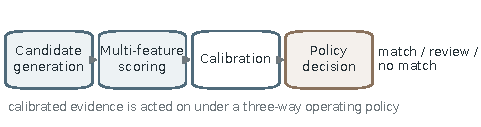
\includegraphics[width=\columnwidth]{figures/system_pipeline.pdf}
\caption{Overall workflow: candidate generation, multi-feature scoring, calibration, and a three-way decision policy.}
\label{fig:pipeline}
\end{figure}

\section{Related Work}
\textbf{Identity linkage and representation.} Fellegi--Sunter linkage introduced match, possible-match, and non-match regions \cite{fellegi1969theory}. Cross-network user linkage extends this setting to heterogeneous social profiles \cite{shu2017uilreview,linkSocial2018}. Neural entity matching and pretrained language models can capture semantic evidence beyond string similarity \cite{barlaug2021survey,li2020ditto}. Our contribution is not a new classifier or embedding; it is the controlled integration of empirical feature/model development with downstream operating-policy selection.

\textbf{Retrieval and abstention.} Blocking controls quadratic comparison cost, but a downstream scorer cannot recover a missed pair \cite{papadakis2021blocking,thirumuruganathan2021deepblocker}. Three-way linkage and reject-option learning explicitly retain uncertainty rather than forcing a binary decision \cite{ouyang2019threeway,chow1970reject,hendrickx2024reject}. Our REVIEW label is an offline system decision; we do not evaluate reviewers.

\textbf{Evolutionary policy search.} GA-based entity-resolution work exists \cite{sun2017gaer}. We therefore make no broad novelty claim for genetic search. Instead, we compare GA with deterministic Sobol search using an identical four-parameter policy, validation data, bounds, objective, and realized evaluation budget.

\section{Evidence and Model Development}
\subsection{Candidate Generation}
We use a normalized local derivative of the public LinkSocial corpus spanning Twitter, Google+, and Instagram \cite{linkSocial2018}. Frozen validity rules retain 36,804 profiles. The eligible cross-platform universe contains 449,149,239 pairs and 29,243 positive links. Deterministic candidate generation yields 12,403 exact-tier pairs and 2,073,842 model-scored pairs, or 2,086,245 workflow candidates. It covers 25,931 positives and misses 3,312, for retrieval recall of 88.6742\% and candidate-space reduction of 99.5355\%. Four same-platform positives are excluded from this denominator. Fig.~\ref{fig:ceiling} shows this split: a downstream scorer cannot recover a pair that candidate generation never presents to it, so the 3,312 missed positives set a hard ceiling on end-to-end recall regardless of classifier quality.

\begin{figure}[t]
\centering
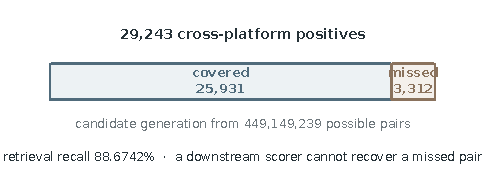
\includegraphics[width=0.72\columnwidth]{figures/candidate_ceiling.pdf}
\caption{Candidate-generation retrieval ceiling over the 29,243 cross-platform positives.}
\label{fig:ceiling}
\end{figure}

\subsection{Empirical Model-Family Choice}
Gradient Boosting was not selected by convention alone. An earlier entity-disjoint development screen compared three families on a 22-feature configuration (Fig.~\ref{fig:model_family}). Validation average precision was 0.9783 for Gradient Boosting, 0.9769 for Random Forest, and 0.9404 for logistic regression, motivating the selected family. These values are historical development evidence only: their feature schema, sampling, and split protocol differ from the final experiment, so they are not used as authoritative test results or combined with Table~\ref{tab:results}.

\begin{figure}[t]
\centering
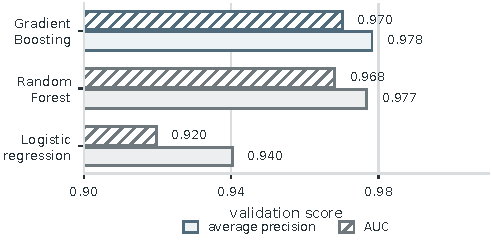
\includegraphics[width=0.85\columnwidth]{figures/model_family_development.pdf}
\caption{Development-stage model-family screen (22-feature configuration, not authoritative V2 evidence).}
\label{fig:model_family}
\end{figure}

\subsection{Multi-Feature Representation}\label{sec:representation}
The broader development program considered identity evidence from usernames, full names, biographies, URL/domain fields, locations, platform context, evidence availability, lexical similarities, and semantic text. The authoritative 17-feature Gradient Boosting model (GB-17) freezes the compatible subset: Jaro, normalized Levenshtein, and token-sort scores for usernames and full names; an unconditional maximum cross-field name similarity; biography Jaccard, length ratio, and availability; location similarity, exactness, and availability; platform agreement; and name length, word-count, and prefix indicators. Missing evidence is encoded deterministically and no feature reads labels, split roles, predecessor scores, or policy decisions.

The semantic-augmented Gradient Boosting model (GB-18) adds exactly one feature: cosine similarity between normalized all-MiniLM-L6-v2 embeddings of profile text assembled from full name, biography, and location. The encoder is fixed and receives no task labels. Thus GB-17 versus GB-18 isolates this semantic cosine; it does not evaluate a general transformer architecture or the full historical feature pool.

For each outer partition, both models use 300 estimators, learning rate 0.05, maximum depth 6, and random state 42. TRAIN retains all positives and a deterministic 3:1 negative sample. An isotonic regressor fitted only on CALIBRATION maps pair scores to $P(\mathrm{match})$ \cite{niculescu2005calibration}.

\section{Business-Informed Three-Way Optimization}
\subsection{From Probability to Operational Action}
The initial policy maps calibrated probabilities to MATCH, REVIEW, or NO\_MATCH with fixed thresholds $t_m=0.98$ and $t_r=0.95$. Earlier fixed-policy experiments exposed the reason for optimization: changing thresholds redistributes uncertain cases among review, false merges, and missed merges. Optimizing classifier discrimination alone cannot choose this operating trade-off.

We encode a \emph{scenario-based remediation-effort objective}. Assumed handling times are 20 minutes for an erroneous merge (FP), 10 minutes for a missed merge (FN), and one minute for review. At the same labor rate these become 33.33, 16.67, and 1.67 THB; normalizing by the FN estimate gives
\begin{equation}
U=2\,FP+FN+0.1\,REVIEW .
\end{equation}
These times and currency values are project design assumptions, not measured company losses, stakeholder-elicited utilities, or production time-study observations. We consequently report component outcomes beside $U$.

\subsection{Controlled Policy Ladder}
The fixed policy (B0) has no fitted parameters. The validation-tuned simple policy (B1) searches only $[t_m,t_r]$ while retaining B0 semantics. The expanded Sobol policy (B2) and expanded genetic policy (B3) share genome $[t_m,t_r,c_p,c_d]$. Probabilities at or above $t_m$ match and probabilities below $t_r$ reject. Within the band $t_r \le p < t_m$, name similarity at least $c_p$ promotes to MATCH, below $c_d$ demotes to NO\_MATCH, and remaining cases stay REVIEW. B1 searches $t_r$ over $[0.50,0.999]$, whereas B2 and B3 search $t_r$ over $[0.50,0.90]$ and $c_d$ over $[0,0.60]$; B1 and B2 are therefore not strictly nested parameter domains.

This ladder gives three contrasts: B0--B1 measures validation selection within the simple-policy domain; B1--B2 measures the transition from the tuned simple policy to the declared expanded four-parameter policy and search domain; B2--B3 isolates optimizer choice under an identical policy class, bounds, objective, validation data, and budget. B2 and B3 receive exactly 12,000 realized objective evaluations per outer partition. The GA uses a population of 60 with seeded selection and Gaussian mutation over 200 evaluated populations; proposals are not deduplicated, so it evaluates 8,414/8,488/8,874 unique parameter vectors (seeds 101/202/303) within the equalized call budget, while Sobol evaluates 12,000 distinct points. Only POLICY\_VALIDATION labels guide selection.

\begin{table}[t]
\caption{Controlled decision-policy ladder.}
\label{tab:policies}
\centering
\begin{tabular}{llllr}
\toprule
ID & Descriptive policy & Params. & Search & Eval.\\
\midrule
B0 & Fixed simple & 0 & None & 0\\
B1 & Validation-tuned simple & 2 & Sobol & 12k\\
B2 & Expanded Sobol & 4 & Sobol & 12k\\
B3 & Expanded genetic & 4 & GA & 12k\\
\bottomrule
\end{tabular}
\end{table}

\section{Leakage-Safe Experimental Design}
Each seed (101, 202, 303) assigns complete entities to TRAIN, CALIBRATION, POLICY\_VALIDATION, or SEALED\_TEST. Cross-role pairs are discarded, giving zero entity overlap. Development labels are role-specific. SEALED\_TEST labels reside in separate artifacts and are unavailable during training, calibration, policy selection, and test prediction.

As Table~\ref{tab:roles} shows, label-free test predictions are canonicalized and SHA-256 hashed into a pre-label freeze manifest after models, calibrators, and policies are frozen and before any test-label access; final evaluation refuses to start without this manifest and re-verifies the prediction hash afterwards. Pre-final validation inspects sealed-label artifacts only by content hash, parquet schema, row count, and label-free pair keys; the ground-truth column is materialized solely inside FINAL\_EVALUATION through a single lazy adapter joined by safe pair key. Process-wide runtime instrumentation records zero pre-final test-label-value materializations for all runs. Independent evaluation recomputes row-level decisions and metrics.

\begin{table}[t]
\caption{Entity-disjoint roles and label availability.}
\label{tab:roles}
\centering
\setlength{\tabcolsep}{3pt}
\begin{tabular}{p{0.24\columnwidth}p{0.36\columnwidth}p{0.24\columnwidth}}
\toprule
Role & Used for & Labels\\
\midrule
Train & GB-17 / GB-18 fitting & yes\\
Calibration & isotonic $P(\mathrm{match})$ & yes\\
Policy val. & B1--B3 threshold search & yes\\
Sealed test & final metrics only & frozen\\
\bottomrule
\end{tabular}
\end{table}

Workflow metrics combine exact-tier MATCH decisions, model-scored candidates, and blocking-missed positives counted as NO\_MATCH. Blocking misses are never passed through the classifier. Reported recall is \emph{decision recall}, $TP/(TP+FN)$, where FN counts positives decided NO\_MATCH (including blocking misses); positives deferred to REVIEW are excluded from this denominator and reported separately in the REVIEW column. We report precision, decision recall, F1, FP, FN, REVIEW, and $U$ as means and sample standard deviations over the three partitions.

\section{Results and Discussion}
\begin{figure}[!t]
\centering
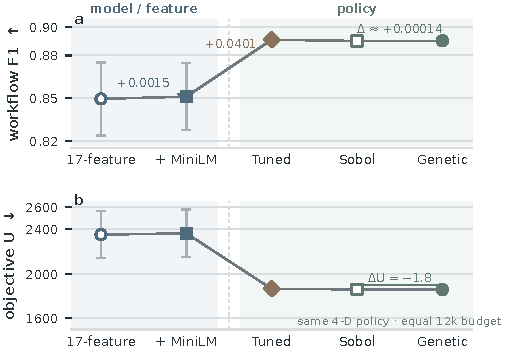
\includegraphics[width=\columnwidth]{figures/controlled_results.pdf}
\caption{Mean $\pm$ sample SD: semantic augmentation changes little, validation tuning gives the major improvement, and equal-budget Sobol and genetic search are nearly equivalent.}
\label{fig:results}
\end{figure}

\begin{table*}[t]
\caption{Authoritative workflow results over three entity-disjoint outer partitions (mean $\pm$ sample SD). Lower $U$ is better.}
\label{tab:results}
\centering
\begin{tabular}{lrrrrrrr}
\toprule
Method & Precision & Recall & F1 & FP & FN & Review & $U$\\
\midrule
GB-17+B0 & 0.9863$\pm$0.0024 & 0.7466$\pm$0.0405 & 0.8494$\pm$0.0257 & 89.0$\pm$25.1 & 2137.3$\pm$211.9 & 366.3$\pm$461.0 & 2352.0$\pm$212.3\\
GB-18+B0 & 0.9870$\pm$0.0080 & 0.7486$\pm$0.0387 & 0.8510$\pm$0.0235 & 88.0$\pm$56.5 & 2171.3$\pm$251.8 & 168.7$\pm$288.7 & 2364.2$\pm$212.0\\
GB-18+B1 & 0.9834$\pm$0.0047 & 0.8146$\pm$0.0008 & 0.8910$\pm$0.0024 & 115.3$\pm$30.1 & 1557.7$\pm$31.1 & 762.3$\pm$178.1 & 1864.6$\pm$45.9\\
GB-18+B2 & 0.9844$\pm$0.0029 & 0.8124$\pm$0.0041 & 0.8901$\pm$0.0016 & 107.7$\pm$21.7 & 1560.3$\pm$32.6 & 843.7$\pm$260.7 & 1860.0$\pm$27.1\\
GB-18+B3 & 0.9844$\pm$0.0029 & 0.8127$\pm$0.0037 & 0.8903$\pm$0.0015 & 107.7$\pm$21.7 & 1557.7$\pm$31.1 & 852.3$\pm$263.9 & 1858.2$\pm$30.0\\
\bottomrule
\end{tabular}
\end{table*}

\textbf{What feature development contributed.} Under fixed operation, adding the MiniLM cosine changes mean workflow F1 from $0.8494\pm0.0257$ to $0.8510\pm0.0235$, while $U$ worsens by 12.2. The single semantic augmentation therefore provides no substantive improvement relative to between-partition variation. This negative result does not negate the multi-feature model: it is consistent with the frozen handcrafted representation already containing the dominant evidence in this test, and it shows that one additional cosine is insufficient to claim semantic benefit.

\textbf{Why policy optimization mattered.} Moving from the fixed policy (B0) to validation-tuned thresholds (B1) raises recall from 0.7486 to 0.8146 and F1 from 0.8510 to 0.8910, while reducing $U$ by 499.6. Mean FN falls by 613.7, but FP rises by 27.3 and REVIEW by 593.7. The result is operational rather than uniformly better: tuning improves the declared objective and F1 by accepting more false-merge and review burden.

\textbf{What policy flexibility and GA achieved.} B1--B2 changes the policy class and its non-nested search domain. The expanded Sobol policy improves mean $U$ by only 4.5 (raw means) and lowers F1 by 0.0009, indicating a small objective-specific trade-off attributable to the combined class-and-domain change rather than added parameters alone. The expanded genetic policy obtains the lowest mean $U$, 1858.2, and F1 0.8903. However, B2 and B3 differ by only 1.8 objective points and 0.00014 F1. GA improves $U$ by 5.5 in seed 101, ties in seed 202, and is 0.1 worse in seed 303. Thus GA successfully searches the operational policy and improves substantially over fixed operation, but the controlled comparison attributes almost all gain to validation-based policy selection rather than to GA specifically.

\textbf{Candidate ceiling.} The 3,312 blocking-missed positives impose an 88.6742\% global retrieval ceiling. In sealed roles the missed counts are 1,034, 1,014, and 1,007. Counting them as workflow FN prevents model-scored metrics from overstating end-to-end recall.

\section{Limitations and Threats to Validity}
The study uses one historical corpus and three deterministic outer partitions, so it does not establish external generalization. Candidate blocking creates a fixed retrieval ceiling and possible selection effects. The model-family screen is historical development evidence and is not directly comparable with the authoritative protocol. The semantic intervention is only one fixed cosine; URL/domain evidence considered during broader development is not part of the final 17-feature schema.

The objective coefficients are assumed remediation effort, not measured economic cost; a different preference can select another operating point. REVIEW is an offline output, with no evaluation of human accuracy, workload, agreement, or latency. No CRM platform, lead scoring, customer conversion, personalization, or downstream agent was tested. GA does not consistently beat equal-budget Sobol in this low-dimensional space. Finally, public hosting was verified, but reuse license, redistribution permission, collection/Terms-of-Service evidence, consent, and ethics documentation were not; release should remain limited to code, configurations, hashes, and aggregates pending clarification.

\section{Conclusion}
Cross-platform identity resolution requires both heterogeneous evidence integration and operational decision control. Empirical development motivated a multi-feature Gradient Boosting scorer; the authoritative ablation finds little additional benefit from one MiniLM cosine. Validation-selected three-way operation produces the main observed improvement over fixed thresholds. Genetic search can optimize the expanded policy under the declared remediation-effort objective, but its outcome is effectively the same as equal-budget Sobol search. The model determines what identity evidence can be inferred; the policy determines how that evidence is acted upon under asymmetric consequences. The result supports controlled, leakage-safe operating-policy selection for profile linkage, not claims about downstream agentic CRM effectiveness.

\bibliographystyle{IEEEtran}
\bibliography{references}
\end{document}
